\subsection{distortion}

In order to get a good image, we added a lens in front of the camera. The addition of the lens has a new influence on the propagation of light during imaging: one is the effect of the shape of the lens itself on the propagation of light, and the other is that during the mechanical assembly process, the lens and the imaging plane are not completely parallel, which also makes the light The position when projected through the lens onto the imaging surface changes.

The \textbf{distortion} (distortion) caused by the shape of the lens is called \textbf{radial distortion}. In the pinhole model, a straight line is projected onto the pixel plane or a straight line. However, in the actual photograph taken, the lens of the camera tends to make a straight line in the real environment become a curve in the picture \footnote{Yes, it is no longer straight, but becomes curved. If you bend inside, it is called barrel distortion; when you bend outward, it is pincushion distortion. }. The closer to the edge of the image, the more obvious this phenomenon is. Since the lenses actually produced are often center-symmetrical, this makes the irregular distortion generally radially symmetrical. They fall into two main categories: \textbf{barrel distortion} and \textbf{pincus distortion}, as shown by \autoref{fig:distortion}.

\begin{figure}[!t]
	\centering
	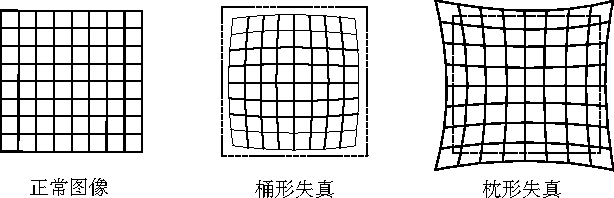
\includegraphics[width=0.7\textwidth]{chapter05/resources/cameraModel/distortion.pdf}
	\caption{Two types of radial distortion.}
	\label{fig:distortion}
\end{figure}

The barrel distortion is due to the fact that the image magnification decreases as the distance from the optical axis increases, while the pincushion distortion is just the opposite. In both distortions, the line that intersects the intersection of the center of the image and the optical axis remains the same shape.

In addition to the shape of the lens, which introduces radial distortion, \textbf{tangential distortion} is introduced in the assembly process of the camera because the lens and the imaging surface cannot be strictly parallel, as shown by \autoref{fig:tangen}.

\begin{figure}[!t]
	\centering
	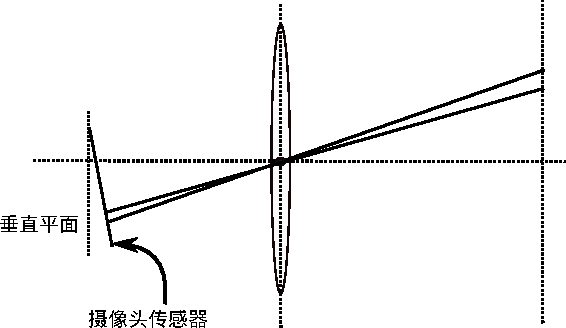
\includegraphics[width=0.7\textwidth]{chapter05/resources/cameraModel/tangen.pdf}
	\caption{Schematic diagram of tangential distortion source.}
	\label{fig:tangen}
\end{figure}

To better understand radial and tangential distortion, we describe the two in more rigorous mathematical form. Consider any point on the \textbf{normalized plane}, $\bm{p}$, whose coordinates are $[x,y]^\mathrm{T}$, or in the form of polar coordinates $[r,\theta]^\mathrm{T}$, where $r$ represents the distance between the point $\bm{p}$ and the origin of the coordinate system, and $\theta$ represents the angle to the horizontal axis. Radial distortion can be seen as a change in the coordinate point along the length, that is, its length from the origin. Tangential distortion can be seen as a change in the coordinate point along the tangential direction, that is, the horizontal angle has changed. It is generally assumed that these distortions are polynomial, namely:

\begin{equation}
\label{eq:distortion} 
\begin{matrix}
x_\mathrm{distorted} = x(1+k_1r^2+k_2r^4+k_3r^6)\\
y_\mathrm{distorted} = y(1+k_1r^2+k_2r^4+k_3r^6)
\end{matrix}.
\end{equation}
Where $[x_\mathrm{distorted}, y_\mathrm{distorted}]^\mathrm{T}$ is the \textbf{normalized coordinate} of the point after the distortion. On the other hand, for \textbf{tangential distortion}, you can use the other two parameters $p_1,p_2$ to correct:
\begin{equation}
\label{eq:tangen} 
\begin{matrix}
x_\mathrm{distorted} = x+2p_1xy+p_2(r^2+2x^2)\\
y_\mathrm{distorted} = y+p_1(r^2+2y^2)+2p_2xy
\end{matrix}. 
\end{equation}

Therefore, the joint \eqref{eq:distortion} and the formula \eqref{eq:tangen}, for a point $\bm{P}$ in the camera coordinate system, we can find this point on the pixel plane by 5 distortion coefficients. The correct location:

\begin{enumerate}
	\item Projects a 3D space point onto a normalized image plane. Let its normalized coordinates be $[x,y]^\mathrm{T}$.
	
	\item calculates radial and tangential distortions for points on the normalized plane.
	\begin{equation}
	\left\{\begin{matrix} x_\mathrm{distorted} =x(1+k_1r^2+k_2r^4+k_3r^6)+2p_1xy+p_2(r^2+2x^2)\\ 
	Y_\mathrm{distorted} = y(1+k_1r^2+k_2r^4+k_3r^6)+p_1(r^2+2y^2)+2p_2xy
	\end{matrix}\right. .
	\end{equation}
	\item Projects the distorted point through the inner parameter matrix to the pixel plane to get the correct position of the point on the image.
	\begin{equation}
	\left\{\begin{matrix} u=f_x x_\mathrm{distorted} + c_x\\ v=f_y y_\mathrm{distorted} + c_y\end{matrix}\right.
	\end{equation}
\end{enumerate}

In the above process of correcting distortion, we used 5 distortion terms. In practical applications, you can flexibly choose to correct the model, for example, only select $k_1, p_1, p_2$ and so on.

In this section, we modeled the camera's imaging process using a pinhole model and described the radial and tangential distortions caused by the lens. In the actual image system, scholars have proposed many other models, such as the camera's affine model and perspective model, and there are many other types of distortion. Considering that ordinary cameras are commonly used in visual SLAM, pinhole models and radial distortion and tangential distortion models are sufficient, so we will not describe other models.

It is worth mentioning that there are two methods of undistorting (or distortion correction). We can choose to dedistort the entire image first, get the distorted image, and then discuss the spatial position of the points on the image. Alternatively, the spatial position before the distortion can be discussed from a certain point on the distorted image according to the distortion equation. Both are feasible, but the former seems to be more common in visual SLAM. Therefore, when an image is dedistorted, we can directly establish a projection relationship with the pinhole model without considering distortion. Therefore, in the discussion that follows, we can directly assume that the image has been dedistorted.

\begin{enumerate}
	\item First, there is a fixed point $P$ in the world coordinate system, and the world coordinates are $\bm{P}_w$.
	\item Since the camera is moving, its motion is described by $\bm{R}, \bm{t}$ or the transformation matrix $\bm{T} \in \mathrm{SE}(3)$. The camera coordinates for $P$ are $\bm{\tilde{P}}_c = \bm{R} \bm{P}_w + \bm{t}$.
	\item The $\bm{\tilde{P}}_c$ component is $X,Y,Z$, and they are projected onto the normalized plane $Z=1$ to get the normalization of $P$. Coordinates: $\bm{P}_c = [X/Z, Y/Z, 1]^\mathrm{T}$\footnote{Note that $Z$ may be less than 1, indicating that the point is behind the normalization plane It may not be imaged on the camera plane and should be checked once in practice. }.
	When \item is distorted, the coordinates of $\bm{P}_c$ after distortion are calculated according to the distortion parameters.
	\item Finally, the normalized coordinates of $P$ pass through the inner parameter and correspond to its pixel coordinates: $\bm{P}_{uv} = \bm{K} \bm{P}_c$.
\end{enumerate}

In summary, we have talked about four coordinates: world coordinates, camera coordinates, normalized coordinates, and pixel coordinates. Ask the reader to clarify their relationship, which reflects the entire imaging process.
